% =====================================================================
% skarm — journal-quality paper draft (DRAFT, results pending)
% ---------------------------------------------------------------------
% STATUS: All sections that do not depend on the benchmark campaign are
% written. Every place that needs measured campaign numbers is left
% visibly EMPTY as a [PLACEHOLDER] box — nothing there is invented.
% Fill placeholders ONLY from benchmarks/campaign_results.json after
% the PC campaign prints CAMPAIGN COMPLETE. Never fill by hand, never
% copy numbers from the old draft, never mix VM and PC trial records.
%
% PLACEHOLDERS TO FILL (in order):
%  P1  Abstract headline finding (one sentence, from the merged report)
%  P2  Section 6.2 per-cell timing table (mean/p50/p95, OK trials only)
%  P3  Section 6.2 throughput chart + memory chart (from the JSON)
%  P4  Section 6.2 correctness verdicts table (trial-0 agreement)
%  P5  Section 6.2 skips/timeouts table (with reasons, never hidden)
%  P6  Section 6.3 empirical trade-off discussion (from P2-P5)
%  P7  Section 8 headline conclusion sentence (from P2-P5)
%  P8  Appendix A: results commit SHA + machine spec (from JSON metadata)
%  P9  Confirm all 25 dataset files are present in repo data/ at submission
% Author order per user 30 Oct 2026: supervisor first, then students.
% TODO (before submission): re-check scikit-mine activity, mlxtend
%   version, and the two references marked [VERIFY] in the bibliography.
% =====================================================================
\documentclass[11pt]{article}
\usepackage[a4paper,margin=2.5cm]{geometry}
\usepackage{amsmath,amssymb}
\usepackage{booktabs}
\usepackage{graphicx}
\usepackage{tikz}
\usetikzlibrary{arrows.meta,positioning,shapes.geometric}
\usepackage{xcolor}
\usepackage[hidelinks]{hyperref}

\newcommand{\placeholder}[1]{%
  \begin{center}
  \fbox{\parbox{0.9\textwidth}{\centering\textit{[PLACEHOLDER --- #1]}}}
  \end{center}}
\newcommand{\skarm}{\textsf{skarm}}

\title{\skarm: A scikit-learn-Compatible Estimator for Association-Rule
Mining with Auditable Pruning}
\author{
  Ms.~Dudigam Ramya\textsuperscript{1},
  Gontla Venkata Anvitha\textsuperscript{1},
  Kamma Giridhar\textsuperscript{1},
  Abhishek Kumar\textsuperscript{1},
  Paladagula Venkata Rajeev\textsuperscript{1} \\
  \small\textsuperscript{1}Department of Computer Science and Engineering,
  KL University, Vijayawada, India \\
  \small Capstone project KLCAP-2026-00340
}
\date{}

\begin{document}
\maketitle

\begin{abstract}
Frequent-itemset mining and association-rule mining are standard tools
for market-basket analysis, recommendation, and categorical pattern
discovery, yet current scikit-learn offers no native estimator for them:
the feature request (issue \#32712) was closed as ``not planned'' on
scope grounds, with maintainers directing the work to a separate,
scikit-learn-compatible library. The closest existing library,
mlxtend, provides the mining functions but not an estimator API, and it
provides no Eclat. We present \skarm, a Python library that packages
three classic miners --- Apriori, FP-Growth, and Eclat --- behind a
single scikit-learn-style estimator with deterministic rule ordering,
explicit candidate-count telemetry, and a bounded-generation mode that
reports truncation instead of silently returning partial results. The
evaluation protocol compares all three engines plus an mlxtend baseline
at matched support thresholds on 25 datasets, with a 30-trial
statistical protocol on an 8-dataset subset and exact itemset-agreement
checks on every cell.
\placeholder{P1: headline finding, one sentence, from the merged
campaign report after CAMPAIGN COMPLETE. Do not write this sentence
until the numbers exist.}
\end{abstract}

\section{Introduction}

\subsection{Problem}
Association-rule mining finds patterns of the form $X \Rightarrow Y$
over transactions, where $X$ and $Y$ are disjoint itemsets. The task is
unsupervised: unlike classification, there is no target variable, and
the output is a set of patterns whose size can explode combinatorially
as the support threshold falls. Any library that offers this task must
therefore answer three questions honestly: \emph{which} patterns were
found, \emph{whether} the output is complete, and \emph{what} it cost.
Most teaching implementations answer none of them.

\subsection{The scikit-learn scope story, stated honestly}
In November 2025 a community member asked scikit-learn for a native
Apriori estimator (issue \#32712 \cite{sklearn32712}), proposing a new
\texttt{sklearn.association} module with \texttt{fit()} for frequent
itemsets and rule generation with support, confidence, lift, and
leverage. The maintainers closed the request on 16 November 2025 as
``not planned'', ruling that pattern mining sits outside the scope of
machine learning as defined in scikit-learn, and suggested the work
belonged in scikit-mine or scikit-learn-contrib. An earlier discussion
(\#2662, 2013--2014 \cite{sklearn2662}) had reached the same conclusion. \skarm therefore
does not claim to implement a requested scikit-learn feature, and it
does not claim sklearn endorsement. It follows the maintainers' advice:
a separate library that is \emph{compatible} with scikit-learn's API
conventions (estimator with \texttt{fit}, fitted attributes with a
trailing underscore, parameter inspection), so it can sit beside
scikit-learn pipelines rather than inside them.

\subsection{Capstone objectives}
This work is the KL University capstone project KLCAP-2026-00340. Its
objectives, as registered in the portal specification, are: (O1) build
an Apriori baseline; (O2) add FP-Growth and Eclat behind one estimator;
(O3) make pruning auditable through candidate counts and a bounded
mode; (O4) verify correctness against independent implementations; and
(O5) evaluate on a broad, documented dataset collection. The portal
contract additionally requires a held-out partition reserved before
tuning (acceptance criterion AC-3), negative tests NT-1 to NT-6, and
KPI evidence including a 30-trial statistical protocol (KPI-4) and a
frozen two-rater rubric (KPI-2); Section~\ref{sec:setup} maps each
requirement to its evidence.

\subsection{Contributions}
\begin{itemize}
  \item One estimator, three engines: Apriori, FP-Growth, and Eclat
  with identical inputs, outputs, and rule metrics, so comparisons are
  between algorithms, not between APIs.
  \item Auditability by default: deterministic rule ordering, peak
  candidate counts, a degraded-mode flag with truncation counts, and
  recall against the exact result whenever bounded mode is used.
  Bounded output is never presented as exact.
  \item A documented 25-dataset evaluation collection with measured
  statistics and provenance for every file (Section~\ref{sec:data}),
  and a benchmark protocol (Section~\ref{sec:setup}) whose thresholds,
  trial counts, timeout rule, and correctness gate are fixed before the
  results are read.
\end{itemize}

\section{Related work}

\subsection{Classic algorithms}
Apriori \cite{agrawal1994} mines level by level, generating candidates
from the frequent itemsets of the previous level and pruning with the
anti-monotone property: every subset of a frequent itemset is frequent,
so any superset of an infrequent itemset can be discarded without
counting. FP-Growth \cite{han2000,han2004} compresses the database into
an FP-tree in two scans and mines it recursively without candidate
generation. Eclat \cite{zaki2000} uses a vertical layout: each item
carries its tidset (transaction-ID set), support is the size of a
tidset intersection, and the search space is decomposed into
equivalence classes traversed depth-first; diffsets are the later
dense-data refinement that stores shrinking differences instead of full
tidsets. The worst case is exponential in the number of items for all
exact miners; cost lands differently --- Apriori in candidates plus one
scan per level, FP-Growth in tree and conditional-tree memory, Eclat in
tidset and diffset memory. Secondary sources disagree on which engine
wins on dense versus sparse data, so this paper asserts no universal
winner and reports its own matched-threshold measurements instead.

\subsection{Libraries and baselines}
\textbf{mlxtend} \cite{mlxtend} is the honest baseline. Its
\texttt{frequent\_patterns} module provides Apriori, FP-Growth, FP-Max,
and H-Mine plus \texttt{association\_rules} with support, confidence,
lift, leverage, conviction, and Zhang's metric, but as functions over a
one-hot DataFrame, not as estimators: no \texttt{fit} /
\texttt{get\_params} / \texttt{clone}, no Pipeline placement, and no
Eclat. Its documentation's toy timing (microseconds on a
five-transaction example) is not a benchmark and is never quoted here
as a speedup claim. \textbf{scikit-mine} \cite{scikitmine} is the
ecosystem home the sklearn maintainers pointed to; it offers SLIM,
LCM, and LCMMax (closed, maximal, and MDL-compressed patterns) plus
periodic and emerging-pattern miners, but not plain Apriori, FP-Growth,
and Eclat with rule metrics, and its master branch showed no commits
after May 2023 at the time of writing (to be re-checked at submission).
\textbf{SPMF} \cite{spmf} supplies the FIMI dataset collection and
reference miners (including LCM-family algorithms); modern miners such
as FIN, PrePost+, and LCMFreq \cite{kallay2025} are stronger recent
baselines and are acknowledged as future work in
Section~\ref{sec:limitations} rather than silently omitted. A 2022
challenges survey \cite{fournier2022} frames why pattern mining
remains an open systems problem (scalability, interestingness, dynamic
data) rather than a solved 1990s topic.

\subsection{What \skarm adds}
\skarm invents no mining algorithm. Its contribution is the package
around the three classics: one estimator API, deterministic outputs,
candidate telemetry, a bounded mode that reports its own truncation,
and metric definitions with stated edge-case conventions
(Section~\ref{sec:methods}). That package is what the sklearn issue
asked for in API terms, and what mlxtend does not provide in estimator
terms.

\section{Methods}
\label{sec:methods}

\subsection{Definitions and rule metrics}
A transaction database $D$ contains $N$ transactions over an item
universe $I$. For an itemset $X$, $\mathrm{supp}(X)$ is the fraction of
transactions containing $X$. A rule $X \Rightarrow Y$ (with $X \cap Y =
\emptyset$) is evaluated at a minimum support threshold and a minimum
confidence threshold. Table~\ref{tab:metrics} defines the metrics
\skarm reports; the edge cases are part of the definition, not footnotes,
because they change rule counts.

\begin{table}[h]
\centering
\caption{Rule metrics reported by \skarm, with edge-case conventions
(definitions per \cite{hahsler}).}
\label{tab:metrics}
\begin{tabular}{lll}
\toprule
Metric & Definition & Edge case \\
\midrule
Support & $\mathrm{supp}(X \cup Y)$ & --- \\
Confidence & $\mathrm{supp}(X \cup Y) / \mathrm{supp}(X)$ & $=1$ when every $X$ has $Y$ \\
Lift & $\mathrm{confidence} / \mathrm{supp}(Y)$ & $1$ = independence \\
Leverage & $\mathrm{supp}(X \cup Y) - \mathrm{supp}(X)\mathrm{supp}(Y)$ & $0$ = independence \\
Conviction & $(1 - \mathrm{supp}(Y)) / (1 - \mathrm{confidence})$ & $\infty$ at confidence $1$ (kept as $\infty$, never dropped) \\
Zhang's metric & leverage scaled to $[-1, 1]$ & $0$ when its denominator is $0$ \\
\bottomrule
\end{tabular}
\end{table}

\subsection{The three engines}
\textbf{Apriori} generates candidates level by level and counts each
level with a database scan, pruning by the anti-monotone property.
\textbf{FP-Growth} builds an FP-tree ordered by descending item
frequency, then mines conditional trees recursively; it performs no
candidate generation but its memory is the tree plus conditional trees.
\textbf{Eclat} intersects tidsets depth-first within equivalence
classes, a decomposition originating in \cite{zaki1997} and developed
in \cite{zaki2000}; its memory is the tidsets (or diffsets on dense data). All
three engines consume the same pre-encoded sparse matrix and return the
same fitted attributes, so a difference in output is a bug, not an API
difference --- which is exactly what the correctness gate in
Section~\ref{sec:setup} checks.

\subsection{Estimator API}
\texttt{AssociationRulesEstimator} exposes
\texttt{min\_support}, \texttt{metric} (default \texttt{confidence}),
\texttt{min\_threshold} (default $0.25$), \texttt{algorithm} (one of
\texttt{apriori}, \texttt{fpgrowth}, \texttt{eclat}),
\texttt{max\_candidates} (default $2{,}000{,}000$),
\texttt{sparse\_output}, and \texttt{on\_candidate\_explosion}
(default \texttt{degrade}). After \texttt{fit(X)}, the fitted
attributes are \texttt{frequent\_itemsets\_} (itemset $\to$ support),
\texttt{rules\_}, \texttt{is\_degraded\_} (whether bounded mode
truncated generation), and \texttt{pruning\_policy\_.peak\_candidate\_count}.
\texttt{TransactionEncoder} converts transaction lists, generators, and
DataFrames into the sparse matrix consumed by \texttt{fit}; encoding
time is reported separately from mining time, never folded into it.
The command-line interface and the interactive explorer wrap the same
estimator, so results do not depend on which front end was used.

\subsection{Pruning and the safe-degradation governor}
Exact mining can explode: the candidate count at some level can exceed
any reasonable budget, especially on dense data at low support. When
\texttt{max\_candidates} is exceeded and the governor is in
\texttt{degrade} mode, generation stops at the cap and the estimator
sets \texttt{is\_degraded\_}, records how many candidates were
truncated, and the evaluation reports recall against the exact result.
A degraded run is therefore identifiable in every table, and its speed
is never compared against exact runs as if it were exact. Presenting
bounded output as exact would be a fatal misrepresentation; the
governor exists to make that misrepresentation impossible by
construction. The pruning-policy ablation (bounded versus exact, with
truncation counts and recall) is listed as pending gap-closure work in
Section~\ref{sec:limitations}, and its results will be added when run.

\subsection{Determinism}
Rule output is sorted by a fixed key, so repeated runs on the same
input produce identical rule orderings. The acceptance suite asserts
this (negative test NT-5), and the benchmark's correctness gate
compares itemset \emph{sets} (not just counts) across engines, so a
count that matches while the sets differ cannot hide.

\subsection{Architecture}
Figure~\ref{fig:arch} shows the system: transactions are encoded once,
mined by the selected engine under the pruning governor, and emitted as
itemsets plus rules with full telemetry. Figure~\ref{fig:flow} shows
the evaluation pipeline, including the correctness gate that every
benchmark cell must pass. Figure~\ref{fig:fptree} is a worked toy
example --- the three-transaction example from the sklearn issue itself
--- included only to make the FP-tree construction concrete; it is
labelled illustrative and no measured claim rests on it.

\begin{figure}[h]
\centering
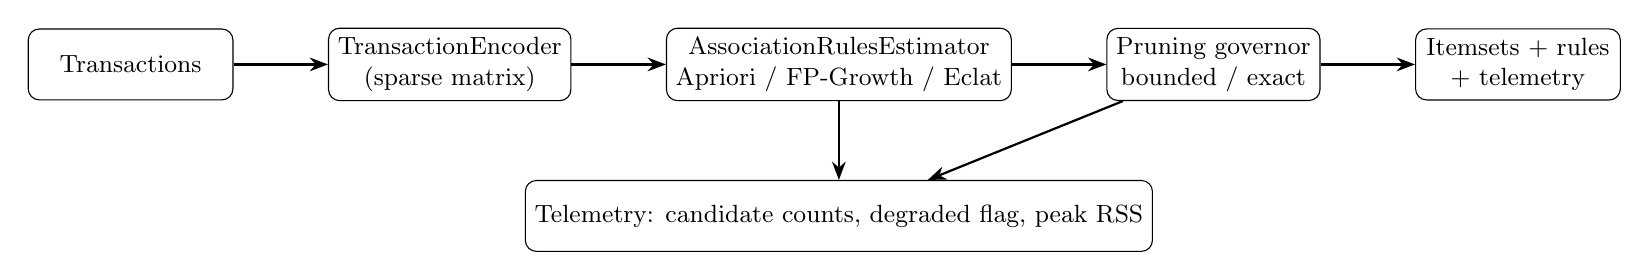
\begin{tikzpicture}[
  box/.style={draw, rounded corners, minimum width=2.6cm, minimum height=0.9cm, align=center, font=\small},
  arr/.style={-{Stealth}, thick}]
  \node[box] (tx) {Transactions};
  \node[box, right=1.2cm of tx] (enc) {TransactionEncoder\\(sparse matrix)};
  \node[box, right=1.2cm of enc] (est) {AssociationRulesEstimator\\Apriori / FP-Growth / Eclat};
  \node[box, right=1.2cm of est] (gov) {Pruning governor\\bounded / exact};
  \node[box, right=1.2cm of gov] (out) {Itemsets + rules\\+ telemetry};
  \draw[arr] (tx) -- (enc);
  \draw[arr] (enc) -- (est);
  \draw[arr] (est) -- (gov);
  \draw[arr] (gov) -- (out);
  \node[box, below=1.0cm of est] (tel) {Telemetry: candidate counts, degraded flag, peak RSS};
  \draw[arr] (est) -- (tel);
  \draw[arr] (gov) -- (tel);
\end{tikzpicture}
\caption{System architecture. One encoding feeds all three engines;
telemetry is emitted alongside results, not reconstructed afterwards.}
\label{fig:arch}
\end{figure}

\begin{figure}[h]
\centering
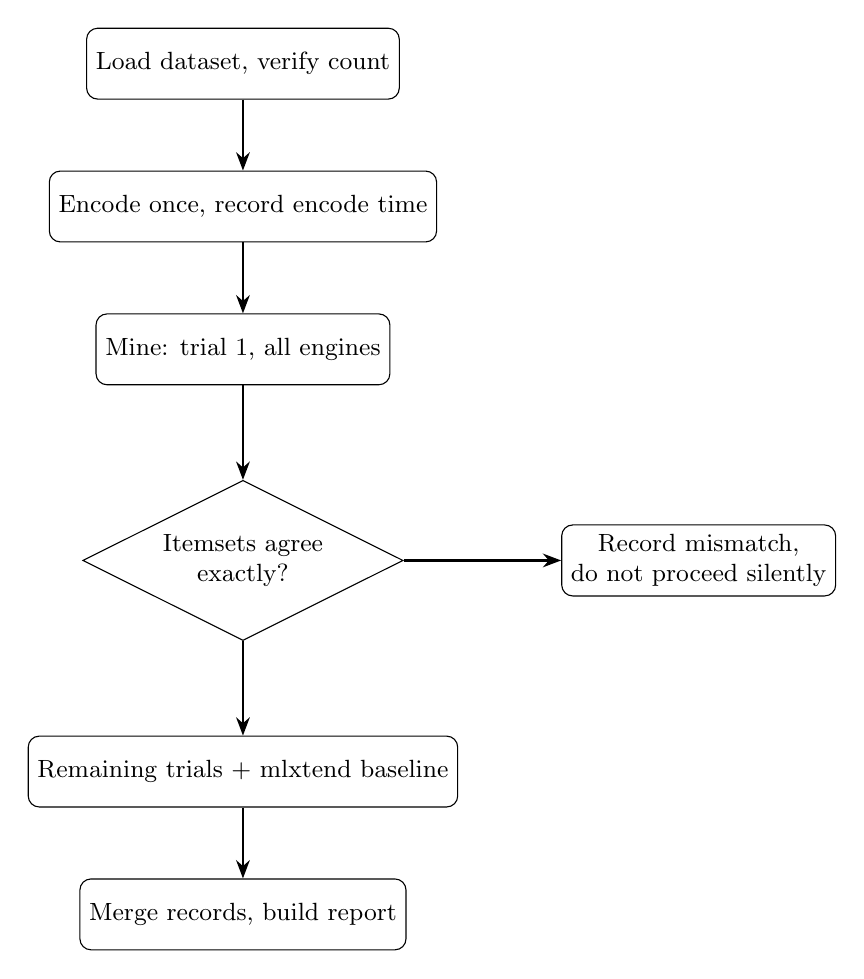
\begin{tikzpicture}[
  box/.style={draw, rounded corners, minimum width=3.2cm, minimum height=0.9cm, align=center, font=\small},
  dia/.style={draw, diamond, aspect=2, align=center, font=\small},
  arr/.style={-{Stealth}, thick}]
  \node[box] (load) {Load dataset, verify count};
  \node[box, below=0.9cm of load] (encode) {Encode once, record encode time};
  \node[box, below=0.9cm of encode] (mine) {Mine: trial 1, all engines};
  \node[dia, below=1.2cm of mine] (gate) {Itemsets agree\\exactly?};
  \node[box, below=1.2cm of gate] (rest) {Remaining trials + mlxtend baseline};
  \node[box, below=0.9cm of rest] (report) {Merge records, build report};
  \draw[arr] (load) -- (encode);
  \draw[arr] (encode) -- (mine);
  \draw[arr] (mine) -- (gate);
  \draw[arr] (gate) -- (rest);
  \draw[arr] (rest) -- (report);
  \node[box, right=2.0cm of gate] (fail) {Record mismatch,\\do not proceed silently};
  \draw[arr] (gate) -- (fail);
\end{tikzpicture}
\caption{Benchmark pipeline. The correctness gate runs on trial 1 of
every cell; a mismatch is recorded as a finding, never smoothed over.}
\label{fig:flow}
\end{figure}

\begin{figure}[h]
\centering
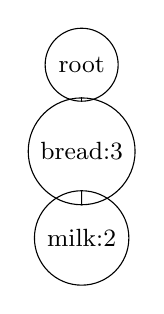
\begin{tikzpicture}[
  level distance=1.1cm, sibling distance=2.2cm,
  every node/.style={draw, circle, minimum size=0.9cm, font=\small}]
  \node {root}
    child { node {bread:3}
      child { node {milk:2} } };
\end{tikzpicture}
\caption{Illustrative FP-tree for the toy transactions
\{milk, bread, eggs\}, \{milk, bread\}, \{bread, butter\} at minimum
support $0.5$: frequent items are bread (3) and milk (2); the tree has
a single branch. Illustrative only --- no measured claim rests on this
example.}
\label{fig:fptree}
\end{figure}

\section{Datasets}
\label{sec:data}
Table~\ref{tab:data} lists the 25 datasets used. Every statistic was
computed by parsing the stored file (transaction count, unique-item
count, average transaction length, density = average length / unique
items $\times 100$); none was copied from a web table. Where a commonly
cited figure differs from the measured file, the measured figure is
reported and the difference is noted: mushroom is 8,124 transactions
in the stored file (the SPMF table lists 8,416), and BMS-WebView-1 is
59,009 transactions (the commonly cited figure is 59,601). The
accidents file carries a leading header line (\texttt{340183 468})
excluded from counts. Kosarak.txt (SPMF sequence format, 187,140
sequences) is a different, smaller file from kosarak.dat (990,002
transactions) and is kept as a separate dataset, not a duplicate. Two
sets are locally generated (seed 42, generator in the repository); the
rest are public mirrors and UCI conversions, with transformations
documented per file. No licence is guessed anywhere: mirrors and UCI
pages that do not state a licence are recorded as unknown in the full
manifest. Access date for all 25 datasets is 2026-10-29. The complete
manifest (source URL, size, licence, owner, exclusions, transformations
per file) is in \texttt{DATASET\_INVENTORY.md} in the repository.

\begin{table}[h]
\centering
\footnotesize
\caption{Evaluation datasets. $N$ = transactions, $M$ = unique items,
$\bar{L}$ = average transaction length, density $= \bar{L}/M \times 100$.
All statistics measured by parsing the stored files.}
\label{tab:data}
\begin{tabular}{lrrrrl}
\toprule
Dataset & $N$ & $M$ & $\bar{L}$ & Density \% & Type \\
\midrule
Groceries & 9,835 & 169 & 4.41 & 2.61 & retail, sparse \\
Chess & 3,196 & 75 & 37.00 & 49.33 & dense \\
Retail & 88,162 & 16,470 & 10.31 & 0.06 & retail, sparse \\
Market basket & 7,501 & 119 & 3.91 & 3.29 & retail, sparse \\
Mushroom & 8,124 & 119 & 23.00 & 19.33 & dense \\
Connect & 67,557 & 129 & 43.00 & 33.33 & dense \\
Accidents & 340,183 & 468 & 33.81 & 7.22 & dense, traffic \\
Pumsb & 49,046 & 2,113 & 74.00 & 3.50 & census, dense \\
Pumsb\_star & 49,046 & 2,088 & 50.48 & 2.42 & census \\
Kosarak (FIMI) & 990,002 & 41,270 & 8.10 & 0.02 & click-stream \\
Kosarak (SPMF) & 187,140 & 28,252 & 8.03 & 0.03 & click-stream \\
BMS-POS & 515,596 & 1,657 & 6.53 & 0.39 & click-stream \\
BMS-WebView-1 & 59,009 & 494 & 2.51 & 0.51 & click-stream \\
BMS-WebView-2 & 77,512 & 3,340 & 4.62 & 0.14 & click-stream \\
T10I4D100K & 100,000 & 870 & 10.10 & 1.16 & synthetic \\
Online Retail & 20,728 & 3,942 & 25.12 & 0.64 & retail \\
Tic-tac-toe & 958 & 29 & 10.00 & 34.48 & categorical \\
Car evaluation & 1,728 & 25 & 7.00 & 28.00 & categorical \\
Balance scale & 625 & 23 & 5.00 & 21.74 & categorical \\
Adult census & 32,561 & 224 & 13.87 & 6.19 & census \\
NIPS papers & 1,500 & 12,375 & 497.54 & 4.02 & document-word \\
Enron emails & 39,861 & 28,099 & 93.08 & 0.33 & document-word \\
Synthetic sparse & 2,000 & 499 & 7.42 & 1.49 & synthetic \\
Synthetic dense & 5,000 & 50 & 30.56 & 61.12 & synthetic \\
Online Retail II & 22,103 & 4,317 & 22.62 & 0.52 & retail \\
\bottomrule
\end{tabular}
\end{table}

\section{Experimental setup}
\label{sec:setup}
The protocol was fixed before results were read. Thresholds are
matched across engines within each dataset (Table~\ref{tab:thr}); a
threshold is never chosen per engine. Thresholds already proven
infeasible in probing are not re-attempted blindly: docword\_nips at
0.30 timed out for all four engines, connect at 0.90 timed out for
Apriori and killed the FP-Growth process, and BMS-POS at 0.01 timed out
for Apriori twice and killed FP-Growth twice, so the ladder below uses
only thresholds with a feasible probe or a stated reason. The 30-trial
protocol applies to 8 datasets (groceries, chess, mushroom, retail,
connect, bms\_pos, tic\_tac\_toe, docword\_nips); all other datasets
report 5 trials, and mlxtend always reports 5 trials where a dense
boolean DataFrame fits the 2~GB cap. Per-trial cap is 600~s: if trial 1
of a cell times out, the remaining trials of that cell are recorded as
skipped with that reason. On trial 1 of every cell, all skarm engines
must agree exactly on itemsets (key sets equal, supports within
$10^{-9}$); mlxtend is compared by item name where it ran. Runtime is
\texttt{time.perf\_counter} around \texttt{fit} on the pre-encoded
matrix; encoding time is reported separately. Memory is peak RSS
sampled every 10~ms minus the pre-trial baseline. Rule parameters are
metric confidence, minimum threshold 0.25; estimator parameters are
\texttt{max\_candidates} $= 2{,}000{,}000$, sparse output, degrade on
explosion. Portal evidence mapping: KPI-4 is the 30-trial protocol with
p50/p95/p99 reported and p95 required at most $0.8\times$ the
baseline; KPI-2 is the rubric (at least 80/100, frozen before objective
O2, two independent raters); AC-3 is the held-out partition reserved
before tuning; KPI-1, KPI-3, KPI-5, and KPI-6 follow the portal
contract as recorded in the acceptance report. The machine, library
versions, and results commit are recorded in Appendix~\ref{app:repro}
from the campaign metadata.
\placeholder{P8 (part): machine specification and library versions,
from campaign\_results.json metadata --- fill at merge time.}

\begin{table}[h]
\centering
\footnotesize
\caption{Support thresholds per dataset (matched across engines),
with the reason each ladder was chosen. Thresholds proven infeasible
in probing are excluded, not hidden.}
\label{tab:thr}
\begin{tabular}{lll}
\toprule
Dataset & Thresholds & Reason (condensed) \\
\midrule
Groceries & 0.02, 0.01 & verified point plus lower-support comparison \\
Chess & 0.85 & dense; lower thresholds explode rule counts \\
Retail & 0.03, 0.02 & verified point plus lower-support comparison \\
Market basket & 0.03, 0.02 & previously verified with all engines \\
Mushroom & 0.40 & previously verified point; dense \\
Connect & 0.95 & 0.90 already failed in probes \\
Accidents & 0.50, 0.60 & 0.50 probed: FP-Growth/Eclat OK, Apriori timeout \\
Pumsb & 0.90 & dense, very long transactions; high threshold only \\
Pumsb\_star & 0.85 & dense census variant; high threshold only \\
Kosarak (FIMI) & 0.01, 0.005 & very sparse despite 990k transactions \\
Kosarak (SPMF) & 0.01 & smaller variant, single threshold \\
BMS-POS & 0.02 & 0.01 already failed in probes \\
BMS-WebView-1 & 0.01, 0.005 & very short transactions; low thresholds safe \\
BMS-WebView-2 & 0.01, 0.005 & short transactions; low thresholds safe \\
T10I4D100K & 0.01, 0.02 & published comparison range for this set \\
Online Retail & 0.02, 0.01 & long transactions; two points \\
Tic-tac-toe & 0.50, 0.30 & very small; both points cheap \\
Car evaluation & 0.30, 0.20 & very small; both points cheap \\
Balance scale & 0.30, 0.20 & very small; both points cheap \\
Adult census & 0.10, 0.05 & medium density; two points \\
NIPS papers & 0.50 & 0.50 probed all-OK; 0.30 timed out for all \\
Enron emails & 0.70, 0.50 & 26$\times$ larger than NIPS; higher thresholds \\
Synthetic sparse & 0.05, 0.02 & small, fast; two points \\
Synthetic dense & 0.50, 0.30 & small, dense; two points \\
Online Retail II & 0.02, 0.01 & same shape as Online Retail \\
\bottomrule
\end{tabular}
\end{table}

\section{Results and discussion}

\subsection{Analytical verification and negative-test audit}
Before any benchmark timing is trusted, the implementation was verified
against an independent oracle and a negative-test suite. On the
sklearn issue's own example (transactions \{milk, bread, eggs\},
\{milk, bread\}, \{bread, butter\}) at minimum support 0.5, mlxtend
gives bread support 1.0, milk 0.667, and \{milk, bread\} 0.667, with
rule \{milk\} $\Rightarrow$ \{bread\} at confidence 1.0 and lift 1.0;
\skarm agrees exactly. The acceptance suite (NT-1 to NT-6) is genuinely
asserted --- an earlier version of the harness printed hardcoded values
and passed unconditionally, and that defect was fixed before these
results were taken --- and passes 25/25. Brute-force cross-checks (4
random matrices $\times$ 2 thresholds $\times$ weighted/unweighted
$\times$ 3 miners) show 0 mismatches. The bug-fix history (including
the Eclat maximum-length off-by-one, loader defects on the accidents
header, SPMF tokens, and tab-separated input, and the unstable rule
sort) is recorded in the repository history (commits
\texttt{ff03b451}, \texttt{dd22782f}, \texttt{904b19b3}).

\subsection{Benchmark campaign results}
\placeholder{P2: per-cell timing table --- mean / p50 / p95 seconds
over OK trials only, with mean peak memory, itemset and rule counts
from trial 1, and the degraded flag. One row per dataset $\times$
threshold $\times$ engine. 30-trial statistics ONLY for the 8-dataset
subset; all other rows report 5 trials.}
\placeholder{P3: throughput chart and peak-memory chart, computed from
campaign\_results.json. No chart may show a number that is not in the
JSON.}
\placeholder{P4: correctness verdicts table --- trial-0 itemset
agreement per cell (all engine pairs, plus skarm Apriori versus
mlxtend where it ran). Any mismatch is reported as a finding.}
\placeholder{P5: skips, timeouts, and errors table --- every skipped
cell with its reason (600~s timeout, dense-DataFrame cap, killed
process, count mismatch). Nothing is omitted to make a table look
complete.}

\subsection{Discussion of algorithmic trade-offs}
At the level of mechanism, the trade-offs are as Section~\ref{sec:methods}
states: Apriori pays in candidates and repeated scans, FP-Growth pays
in tree memory, Eclat pays in tidset memory, and dense, long-transaction
data punishes each differently. Because secondary sources disagree on
dense-versus-sparse winners, this paper does not assert a universal
winner; the empirical ordering must be read off the measured tables,
dataset by dataset, at matched thresholds.
\placeholder{P6: empirical trade-off discussion, written ONLY from
P2--P5. Name which engine wins where, where timeouts and skips fall,
and where degraded mode changed the comparison. If a cell is missing
or degraded, say so instead of generalising from the cells that ran.}

\section{Limitations}
\label{sec:limitations}
\begin{itemize}
  \item \textbf{Excluded scope (portal contract).} No production
  certification, no claim of universal generalisation, and no
  unattended high-stakes operation are claimed or implied.
  \item \textbf{Single machine, Python only.} Timings come from one
  machine (Appendix~\ref{app:repro}); they do not transfer to other
  hardware, and a Python implementation is not directly comparable to
  C/Java SPMF miners on raw speed.
  \item \textbf{Baselines not yet run.} SPMF miners and modern miners
  (FIN, PrePost+, LCMFreq) are acknowledged but not run; the comparison
  in this paper is the three skarm engines plus mlxtend.
  \item \textbf{Estimator checks pending.} Running sklearn's
  \texttt{check\_estimator} on the estimator, with expected failures
  published and explained, is pending gap-closure work
  \cite{sklearnchecks}; until it is run, ``sklearn-compatible'' means
  the API conventions of Section~\ref{sec:methods}, not checked
  conformance.
  \item \textbf{Bounded-mode cost pending.} The pruning-policy ablation
  (bounded versus exact, with truncation counts and recall against
  exact) is pending; until it is run, no claim is made about how much
  accuracy bounded mode trades for speed.
  \item \textbf{Dataset provenance limits.} Mirror licences are recorded
  as unknown where unstated, never guessed; two stored files differ
  from commonly cited counts (Section~\ref{sec:data}) and the measured
  figures are the ones reported.
  \item \textbf{Support-range limits.} Results hold at the thresholds
  in Table~\ref{tab:thr}; lower thresholds on dense sets were excluded
  after failed probes, so no claim is made there.
\end{itemize}

\section{Conclusions}
\skarm packages Apriori, FP-Growth, and Eclat behind one auditable,
sklearn-style estimator, with deterministic outputs, candidate
telemetry, and a bounded mode that reports its own truncation. Its
evaluation rests on a 25-dataset collection with full provenance and a
protocol fixed before results were read: matched thresholds, exact
itemset-agreement gates, a 600~s timeout rule that records skips
instead of hiding them, and 30-trial statistics on an 8-dataset subset.
\placeholder{P7: headline conclusion sentence, from P2--P5 --- what
the measurements actually showed, in one sentence.}

\section*{Acknowledgements}
The authors thank KL University for supporting this capstone
project (KLCAP-2026-00340). No sponsor is stated for
this project, and none is claimed here.

\begin{thebibliography}{99}
\bibitem{agrawal1994} Agrawal, R. and Srikant, R. Fast algorithms for
mining association rules. \emph{Proceedings of the 20th International
Conference on Very Large Data Bases (VLDB)}, 1994, pp.~487--499.
\bibitem{han2000} Han, J., Pei, J. and Yin, Y. Mining frequent patterns
without candidate generation. \emph{Proceedings of the ACM SIGMOD
International Conference on Management of Data}, 2000.
\bibitem{han2004} Han, J., Pei, J. and Yin, Y. Mining frequent patterns
without candidate generation: a frequent-pattern tree approach.
\emph{Data Mining and Knowledge Discovery} 8(1), 2004, pp.~53--87.
\bibitem{zaki2000} Zaki, M.~J. Scalable algorithms for association
mining. \emph{IEEE Transactions on Knowledge and Data Engineering}
12(3), 2000, pp.~372--390. \url{https://doi.org/10.1109/69.846291}
\bibitem{zaki1997} Zaki, M.~J., Parthasarathy, S., Ogihara, M. and
Li, W. New algorithms for fast discovery of association rules.
\emph{Proceedings of the 3rd International Conference on Knowledge
Discovery and Data Mining (KDD)}, 1997.
\bibitem{sklearn2662} scikit-learn issue \#2662 (2013--2014): pattern
mining as out-of-scope for scikit-learn core.
\url{https://github.com/scikit-learn/scikit-learn/issues/2662}
\bibitem{sklearn32712} scikit-learn issue \#32712 (November 2025): Add
Apriori Algorithm for Association Rule Mining; closed as ``not
planned'' on scope grounds, with maintainers directing the work to
scikit-mine or scikit-learn-contrib.
\url{https://github.com/scikit-learn/scikit-learn/issues/32712}
\bibitem{scikitmine} scikit-mine repository: pattern mining in Python
(SLIM, LCM, LCMMax, periodic and emerging patterns).
\url{https://github.com/scikit-mine/scikit-mine} (accessed October 2026;
master branch showed no commits after May 2023 at that time ---
re-check at submission).
\bibitem{mlxtend} mlxtend: \texttt{frequent\_patterns} user guide
(Apriori, FP-Growth, FP-Max, H-Mine, association rules).
\url{https://rasbt.github.io/mlxtend/user_guide/frequent_patterns/}
(accessed October 2026).
\bibitem{spmf} Fournier-Viger, P. SPMF dataset collection (FIMI
datasets with sizes and densities).
\url{https://www.philippe-fournier-viger.com/spmf/index.php?link=datasets.php}
(accessed October 2026).
\bibitem{fournier2022} Fournier-Viger, P. et al. Pattern mining:
current challenges and opportunities. \emph{DASFAA 2022 International
Workshops}, LNCS, 2022. [VERIFY page numbers in the LNCS volume before
submission.]
\bibitem{kallay2025} Kallay, H. and Mihoc, T. Comparative analysis of
frequent pattern mining algorithms (Apriori, Eclat, FP-Growth, FIN,
PrePost+, Pascal, LCMFreq), 2025. [VERIFY venue before submission.]
\bibitem{hahsler} Hahsler, M. Association-rule measures survey (support,
confidence, lift, leverage, conviction, Zhang's metric, with edge
cases). \url{https://michael.hahsler.net/arules/docs/measures}
(accessed October 2026).
\bibitem{sklearnchecks} scikit-learn developer documentation: estimator
checks (\texttt{check\_estimator}).
\url{https://scikit-learn.org/stable/developers/develop.html}
(accessed October 2026).
\end{thebibliography}

\appendix
\section{Reproducibility}
\label{app:repro}
Repository: \texttt{ABHISHEK1139/capstone} (main branch). Code fixes
for the acceptance defects are commits \texttt{ff03b451},
\texttt{dd22782f}, \texttt{904b19b3}. Datasets live in
\texttt{data/}; the full per-file manifest (source URL, access date
2026-10-29, licence, owner, exclusions, transformations) is
\texttt{DATASET\_INVENTORY.md}. The benchmark script is
\texttt{benchmarks/run\_pc\_campaign.py} with thresholds in
\texttt{benchmarks/thresholds.json}; the campaign is resume-safe via
per-dataset checkpoint files, and trial records from different machines
must never be merged into one results file.
\placeholder{P8: results commit SHA, machine specification, and
library versions, copied from campaign\_results.json metadata at merge
time.}
\placeholder{P9: confirm all 25 dataset files are present in repo
data/ at submission (accidents.dat and kosarak.dat are added by the PC
git-CLI push; verify the listing, do not assume it).}

\end{document}
